\documentclass{article}

\usepackage{graphicx}
\usepackage{tikz}
\usepackage{tikzsymbols}
\usetikzlibrary{calc,patterns,shapes.geometric}
\pagestyle{empty}
\usepackage[margin=0pt]{geometry}
\geometry{papersize={14in,12in}}

\def\centerarc[#1](#2)(#3:#4:#5){\draw[#1] ($(#2)+({#5*cos(#3)},{#5*sin(#3)})$) arc (#3:#4:#5);}

\begin{document}
	\begin{figure}
		\centering
		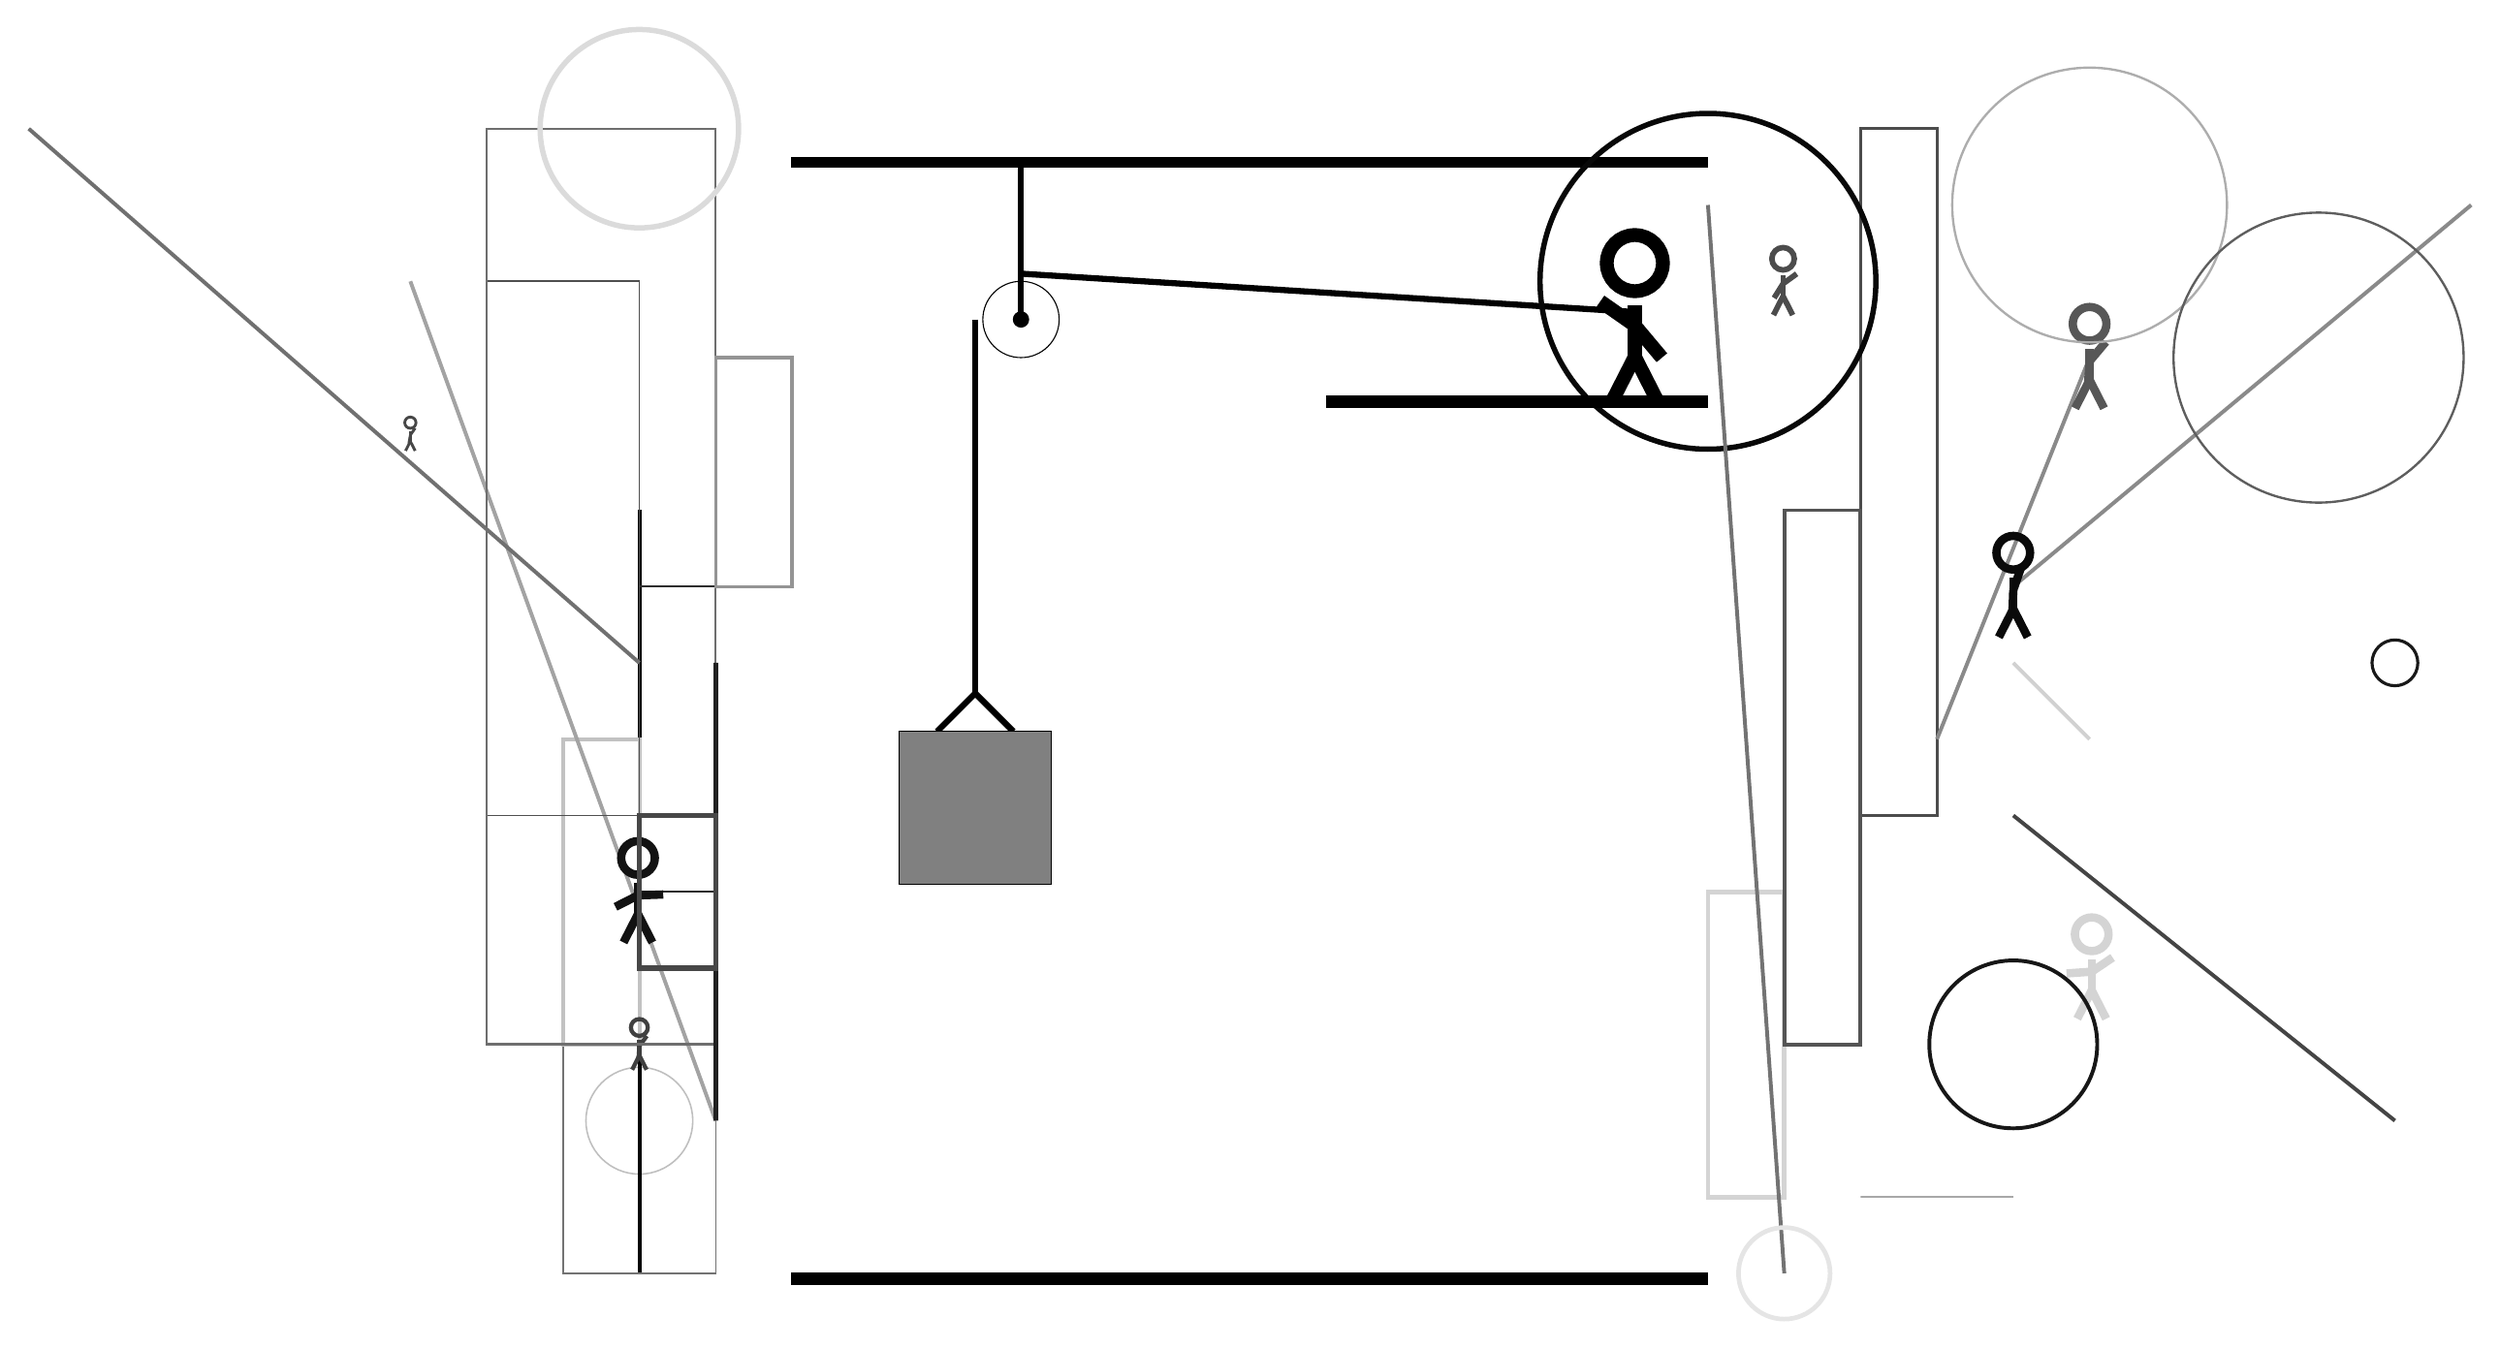
\begin{tikzpicture}
			%%%%% START %%%%%
			
			\draw[fill=black] (-2, 11.5) rectangle (10, 11.625);
			
			\draw (1, 9.5) circle (0.5);
			\draw[fill=black] (1, 9.5) circle (0.1);
			\draw[line width=0.8mm] (1, 11.5) -- (1, 9.5);
			
			\draw[line width=0.8mm](-0.1, 4.1) --  (0.4, 4.6) -- (0.9, 4.1);
			\draw[fill=black!50] (-0.6, 4.1) rectangle (1.4, 2.1);
			
			\draw[line width=0.8mm](0.4, 9.5) -- (0.4, 4.6);
			\centerarc[line width=0.8mm](1, 9.5)(90:180:0.6)
			\draw[line width=0.8mm](1, 10.1) -- (9, 9.6);
			
			\node[line width=0.4mm, color=black!17] at (15, 1) {\Strichmaxerl[6][4][34]};
			
			\draw [line width=0.7mm, color=black!58](-9, 3) circle (0.0);
			\draw [line width=0.2mm, color=black!25](-4, -1) circle (0.7);
			\draw[line width=0.5mm, color=black!46](14, 6) -- (20, 11);
			
			\draw[line width=0.4mm, color=black!70] (12, 3) rectangle (13, 12);
			\draw[line width=0.5mm, color=black!46](15, 9) -- (13, 4);
			\draw[line width=0.5mm, color=black!99](-4, 7) -- (-4, -3);
			\draw [line width=0.7mm, color=black!97](10, 10) circle (2.2);
			\draw[line width=0.2mm, color=black!55] (-3, -3) rectangle (-5, 0);
			\draw[line width=0.6mm, color=black!17] (11, 2) rectangle (10, -2);
			
			\draw[line width=0.5mm, color=black!55](10, 11) -- (11, -3);
			\draw[line width=0.5mm, color=black!24] (-4, 0) rectangle (-5, 4);
			\node[line width=0.7mm, color=black!72] at (-7, 8) {\Strichmaxerl[2][80][56]};
			
			\node[line width=0.4mm, color=black!96] at (14, 6) {\Strichmaxerl[6][88][71]};
			\draw[line width=0.5mm, color=black!36](-3, -1) -- (-7, 10);
			\node[line width=0.5mm, color=black!66] at (15, 9) {\Strichmaxerl[6][86][50]};
			\draw [line width=0.4mm, color=black!90](19, 5) circle (0.3);
			\draw[line width=0.5mm, color=black!73](14, 3) -- (19, -1);
			\node[line width=0.3mm, color=black!70] at (11, 10) {\Strichmaxerl[4][58][36]};
			
			\node[line width=0.7mm, color=black!75] at (-4, 0) {\Strichmaxerl[3][86][54]};
			\draw[line width=0.2mm, color=black!82] (-4, 6) rectangle (-3, 2);
			\draw [line width=0.6mm, color=black!10](11, -3) circle (0.6);
			
			\draw [line width=0.5mm, color=black!91](14, 0) circle (1.1);
			\node[line width=0.4mm, color=black!93] at (-4, 2) {\Strichmaxerl[6][27][2]};
			\draw[line width=0.5mm, color=black!67] (12, 0) rectangle (11, 7);
			\draw[line width=0.2mm, color=black!69] (-4, 3) rectangle (-6, 10);
			\draw[line width=0.3mm, color=black!57] (-3, 12) rectangle (-6, 0);
			\draw[line width=0.7mm, color=black!87] (-3, 5) rectangle (-3, -1);
			\draw[line width=0.3mm, color=black!34] (12, -2) rectangle (14, -2);
			\draw [line width=0.3mm, color=black!32](15, 11) circle (1.8);
			\draw [line width=0.3mm, color=black!63](18, 9) circle (1.9);
			
			\draw[line width=0.5mm, color=black!18](14, 5) -- (15, 4);
			\draw [line width=0.7mm, color=black!14](-4, 12) circle (1.3);
			
			\draw[line width=0.5mm, color=black!56](-4, 5) -- (-12, 12);
			\draw[line width=0.7mm, color=black!72] (-4, 3) rectangle (-3, 1);
			\draw[line width=0.4mm, color=black!42] (-2, 9) rectangle (-3, 6);
			
			
			\node at (9, 9.5) {\Strichmaxerl[10][-35][-50]};
			\draw[fill=black] (5, 8.5) rectangle (10, 8.35);
			
			\draw[fill=black] (-2, -3) rectangle (10, -3.15);
			
			%%%%% END %%%%%
		\end{tikzpicture}
	\end{figure}	
\end{document}